\documentclass{training}
% Filigrane PAR MODULE : \uxfond (PNG A4 dilue 30 %). Cadre noir vectoriel commun.
% Proportions original 744 px : marge 20/744, trait 1/744. Exterieur BLANC.
% Cadre via eso-pic +\put (coordonnees absolues) — pas de remember picture (decalage).
\usepackage{eso-pic}

\providecommand{\uxfond}{../../resources/fond/norme_fond_paliers_30.png}

\newlength{\uxmargin}
\newlength{\uxthick}
\newlength{\uxinnerw}
\newlength{\uxinnerh}
\setlength{\uxmargin}{0.02688\paperwidth}% 20/744
\setlength{\uxthick}{0.001344\paperwidth}% 1/744
\setlength{\uxinnerw}{\dimexpr\paperwidth-2\uxmargin-2\uxthick\relax}
\setlength{\uxinnerh}{\dimexpr\paperheight-2\uxmargin-2\uxthick\relax}

% Contenu strictement a l'interieur du trait (+ jour confortable).
\geometry{%
  includeheadfoot,
  left=22mm,
  right=22mm,
  top=20mm,
  bottom=18mm,
  headheight=30pt,
  headsep=5mm,
  footskip=12mm%
}

\AddToShipoutPictureBG{%
  \AtPageLowerLeft{%
    % Fond blanc page entiere
    \put(0,0){\color{white}\rule{\paperwidth}{\paperheight}}%
    % Filigrane module a l'interieur du cadre
    \put(\LenToUnit{\dimexpr\uxmargin+\uxthick\relax},\LenToUnit{\dimexpr\uxmargin+\uxthick\relax}){%
      \includegraphics[width=\uxinnerw,height=\uxinnerh]{\uxfond}}%
    % Cadre noir : bas, haut, gauche, droite
    \put(\LenToUnit{\uxmargin},\LenToUnit{\uxmargin}){%
      \color{black}\rule{\dimexpr\paperwidth-2\uxmargin\relax}{\uxthick}}%
    \put(\LenToUnit{\uxmargin},\LenToUnit{\dimexpr\paperheight-\uxmargin-\uxthick\relax}){%
      \color{black}\rule{\dimexpr\paperwidth-2\uxmargin\relax}{\uxthick}}%
    \put(\LenToUnit{\uxmargin},\LenToUnit{\uxmargin}){%
      \color{black}\rule{\uxthick}{\dimexpr\paperheight-2\uxmargin\relax}}%
    \put(\LenToUnit{\dimexpr\paperwidth-\uxmargin-\uxthick\relax},\LenToUnit{\uxmargin}){%
      \color{black}\rule{\uxthick}{\dimexpr\paperheight-2\uxmargin\relax}}%
  }%
}

\makeatletter
\fancyhf{}
\fancyheadoffset{0pt}
\renewcommand{\headrulewidth}{0pt}
\lhead{\parbox[t]{0.56\textwidth}{\RaggedRight\footnotesize\sloppy\@title}}
\rhead{\parbox[t]{0.36\textwidth}{\RaggedLeft\footnotesize\sloppy\@subtitle}}
\cfoot{\thepage}
% Coupures : underscore et slash dans les noms de fichiers / consignes
\DeclareRobustCommand{\_}{\textunderscore\allowbreak}
\makeatother

% Evite les depassements de longues lignes (Github, Name_FirstName_...)
\sloppy
\emergencystretch=3em
\hbadness=10000

% Sommaire type 42 : chapitres seulement
\setcounter{tocdepth}{0}
\renewcommand{\cftchappresnum}{}
\renewcommand{\cftchapaftersnum}{}
\setlength{\cftchapnumwidth}{2.0em}
\setlength{\cftbeforechapskip}{0.35em}
\cftsetindents{chapter}{0em}{2.0em}


\begin{document}

\schoollogo{../../resources/jeunecrack.png}
\title{The Olympics}
\subtitle{Piscine UX/UI --- UX}
\member{Piscine UX/UI}{https://github.com/01-edu/UX-UI}
\summary{Ideation, flow, prototype, motion, and a test.}
\version{1.0}
\prerequisite{The previous module of this piscine, or none if this is your first.}
\maketitle

\newpage
\tableofcontents
\newpage


\chapter{Instructions}

The foreword is not an exercise. It will not be graded. The exercises start at the next chapter, from the easiest contract to the hardest. A later exercise is not taken into account if an earlier one does not hold.

Only what is in the turn-in directory of an exercise is looked at. Do not add files that the exercise does not name. The name of a deliverable follows the pattern in the exercise: \texttt{Name\_FirstName\_DeliverableName\_Date\_VersionNumber}.

You will not be given the gesture. The examples in an exercise sometimes carry a constraint that the sentence does not repeat. Read them. Your other references are the manual of the tool you picked, the person sitting next to you, and the links printed in the exercise.

The order is the order of the quest. Skipping a step because a later screen looks more interesting produces a screen nobody can explain.

\subsection*{About the pictures}

The mark on the cover is the project logo. The picture in the foreword is the illustration of this module. The pale ground behind the text is the page watermark. None of them is a hint.

\subsection*{About machines that write}

You may use a tool to look up a term, the way you would use a dictionary. You may not replace an interview, a test, or a file with a generated text and sign it. If you cannot point at the person, the screen, or the line you claim, the exercise is not done.


\chapter{Foreword}

In 1972 Otl Aicher reduced a Games to a set of pictograms that a visitor could read without a shared language. Mexico 1968, under Lance Wyman, had already shown that an identity can be a system rather than a mascot. Look at the pictures if you want. The exercises still ask you to ideate, not to trace those signs.

\begin{center}
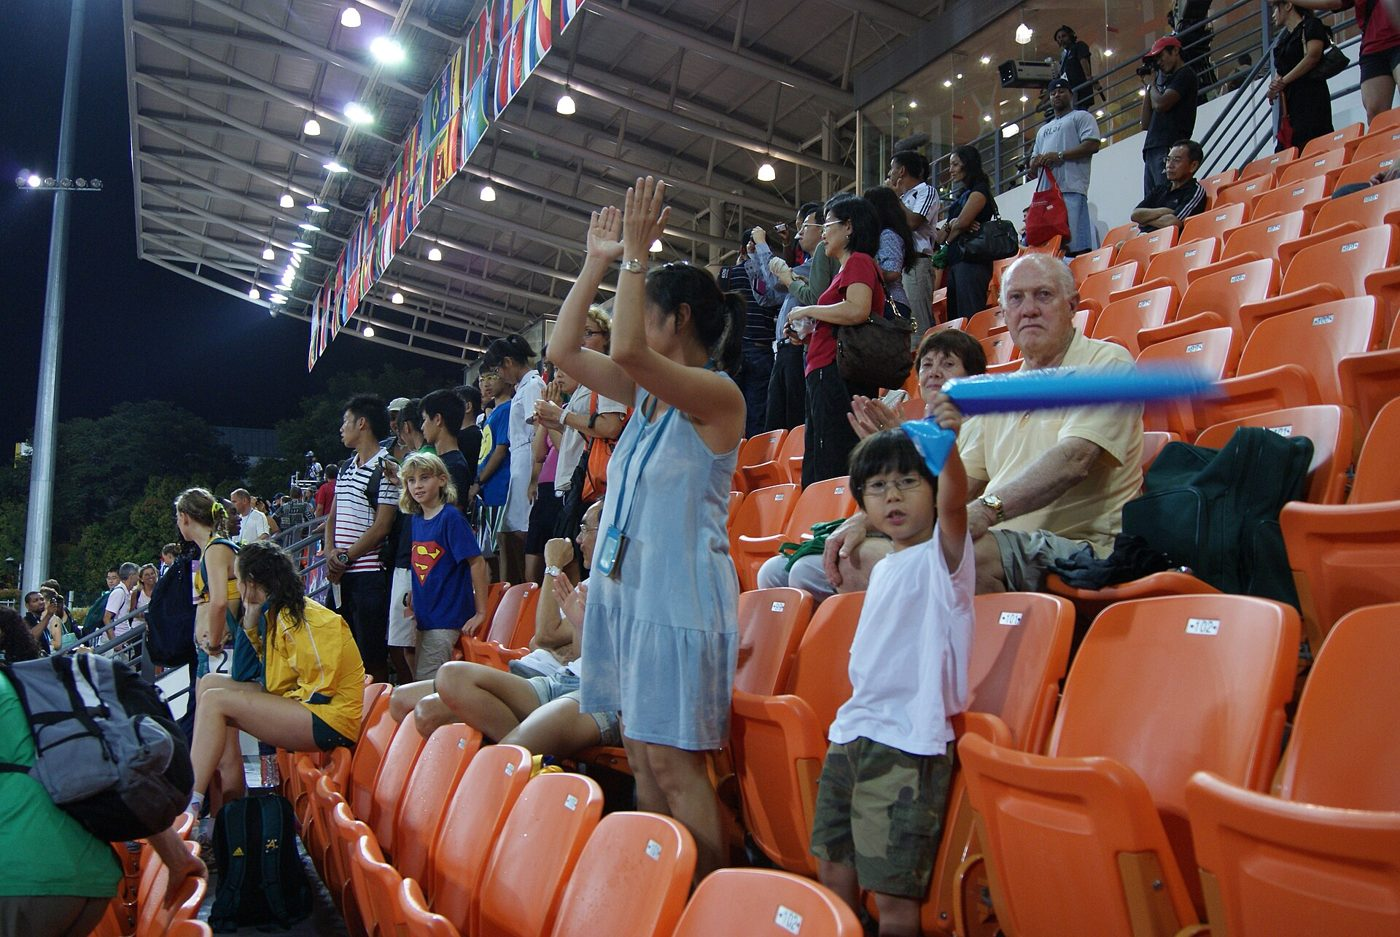
\includegraphics[width=0.78\textwidth,height=0.32\textheight,keepaspectratio]{../../resources/intros/UX-03-the-olympics.jpg}\\[0.4em]
{\footnotesize Picture: Jacklee / CC BY-SA 4.0}
\end{center}

Recommended watching. The videos are context. They are not the deliverable.
\begin{itemize}
\item UX - Introduction \& Quest n°1, 01Edu \url{https://www.youtube.com/watch?v=UbE6WMeuvQg&list=PLHyAJ_GrRtf-RAtfngbRrFh1XDTnyXFDe}
\end{itemize}

\chapter{Exercise 00: UX IV - Ex 1 - Ideation}
\exnumber{00}
\extitle{UX IV - Ex 1 - Ideation}
\exfiles{ex00/zip archive, named Name\_FirstName\_DeliverableName\_Date\_VersionNumber}
\exauthorize{Those named in the exercise}
\makeheaderfiles

\textbf{Context:}

The Olympics committee calls on you to get fresh ideas for the next Olympic Games.

You'll team up by groups of 3 and focus each on one problem statement.

You'll get guidelines and suggestions to run ideation workshops, and bring your ideas to life with three different prototypes, that you will animate and test.

\textbf{Instructions:}

Let's be creative!

Organize and run an ideation workshop with 4 - 8 participants to find ideas to solve this problem statement:

\textbf{How might we create a digital sport anyone (including athletes, non-athletes, disabled) could play between now and the next Olympics edition?}

A is leader, B is time-keeper and C focuses on logistics

\textbf{Deliverables:}

\begin{itemize}
\item A PDF document with the ideation workshop script
\item Pictures of the ongoing workshop
\item A PDF document that represents the main concept out of the workshop
\item Upload the documents on Github, in a zip folder named "ProjectTitle\_Name\_FirstName", with all project deliverables as follows: "Name\_FirstName\_DeliverableName\_Date\_VersionNumber".  For example, the first deliverable can be named as "Doe\_John\_MidFiPrototype\_05242024\_V1".
\item Add a title within all written documents.
\item Pay attention to the global aspect of the deliverables. They must be clear, simple and easy to read. You can get inspiration on canva.com but don't overload your design with too much details!
\end{itemize}

\textbf{Resources:}

\begin{itemize}
\item Where good ideas come from \url{https://www.ted.com/talks/steven_johnson_where_good_ideas_come_from}
\item Creative Confidence - Book by Tom Keller \url{https://booksvooks.com/creative-confidence-unleashing-the-creative-potential-within-us-all-pdf.html}
\item Sketching (podcast) \url{https://www.usersknow.com/podcast/2016/10/10/ua1wdsszhx2pemugxc1e0qj0a3l9cs}
\item 13 unusual brainstorming methods that work \url{http://www.huffingtonpost.com/young-entrepreneur-council/13-unusual-brainstorming_b_3880619.html}
\item 3 proven methods to organize a brainstorming session \url{https://uxdesign.cc/brainstorm-79e51f20f313}
\item Effective brainstorming (without feeling lost) \url{https://uxdesign.cc/effective-brainstorming-without-being-lost-b68750bbfac5?sk=5d5a332f7e3f2a43364c031b01b13229}
\item The myth of brainstorming \url{https://uxdesign.cc/the-myth-of-brainstorming-8517e02facc0?sk=995d601cbf988d574e86dd71364cb92f}
\item Ideation method: Worst possible idea \url{https://www.interaction-design.org/literature/article/learn-how-to-use-the-best-ideation-methods-worst-possible-idea}
\item Up to you to find more!
\end{itemize}


\chapter{Exercise 01: UX IV - Ex 2 - Ideation}
\exnumber{01}
\extitle{UX IV - Ex 2 - Ideation}
\exfiles{ex01/zip archive, named Name\_FirstName\_DeliverableName\_Date\_VersionNumber}
\exauthorize{Those named in the exercise}
\makeheaderfiles

\textbf{Instructions:}

Let's be creative!

Organize and run an ideation workshop with 4 - 8 participants to find ideas to solve this problem statement:

\textbf{How might we provide relevant and on-demand information about the environmental and social impact of the Olympics through our platform?}

B is leader, C is time-keeper and A focuses on logistics.

Pay attention not to use the same ideation technique as in Ex 1!

\textbf{Deliverables:}

\begin{itemize}
\item A PDF document with the ideation workshop script
\item Pictures of the ongoing workshop
\item A PDF document that represents the main concept out of the workshop
\item Upload the documents on Github, in a zip folder named "ProjectTitle\_Name\_FirstName", with all project deliverables as follows: "Name\_FirstName\_DeliverableName\_Date\_VersionNumber".  For example, the first deliverable can be named as "Doe\_John\_MidFiPrototype\_05242024\_V1".
\item Add a title within all written documents.
\item Pay attention to the global aspect of the deliverables. They must be clear, simple and easy to read. You can get inspiration on canva.com but don't overload your design with too much details!
\end{itemize}

\textbf{Resources:}

\begin{itemize}
\item Where good ideas come from \url{https://www.ted.com/talks/steven_johnson_where_good_ideas_come_from}
\item Creative Confidence - Book by Tom Keller \url{https://booksvooks.com/creative-confidence-unleashing-the-creative-potential-within-us-all-pdf.html}
\item Sketching (podcast) \url{https://www.usersknow.com/podcast/2016/10/10/ua1wdsszhx2pemugxc1e0qj0a3l9cs}
\item 13 unusual brainstorming methods that work \url{http://www.huffingtonpost.com/young-entrepreneur-council/13-unusual-brainstorming_b_3880619.html}
\item 3 proven methods to organize a brainstorming session \url{https://uxdesign.cc/brainstorm-79e51f20f313}
\item Effective brainstorming (without feeling lost) \url{https://uxdesign.cc/effective-brainstorming-without-being-lost-b68750bbfac5?sk=5d5a332f7e3f2a43364c031b01b13229}
\item The myth of brainstorming \url{https://uxdesign.cc/the-myth-of-brainstorming-8517e02facc0?sk=995d601cbf988d574e86dd71364cb92f}
\item Ideation method: Worst possible idea \url{https://www.interaction-design.org/literature/article/learn-how-to-use-the-best-ideation-methods-worst-possible-idea}
\item Up to you to find more!
\end{itemize}


\chapter{Exercise 02: UX IV - Ex 3 - Ideation}
\exnumber{02}
\extitle{UX IV - Ex 3 - Ideation}
\exfiles{ex02/zip archive, named Name\_FirstName\_DeliverableName\_Date\_VersionNumber}
\exauthorize{Those named in the exercise}
\makeheaderfiles

\textbf{Instructions:}

Let's be creative!

Organize and run an ideation workshop with 4 - 8 participants to find ideas to solve this problem statement:

\textbf{How might we help sports fans organize local Olympic Games in between 2 international editions?}

C is leader, A is time-keeper and B focuses on logistics.

Pay attention not to use the same ideation technique as in ex 2!

\textbf{Deliverables:}

\begin{itemize}
\item A PDF document with the ideation workshop script
\item Pictures of the ongoing workshop
\item A PDF document that represents the main concept out of the workshop
\item Upload the documents on Github, in a zip folder named "ProjectTitle\_Name\_FirstName", with all project deliverables as follows: "Name\_FirstName\_DeliverableName\_Date\_VersionNumber".  For example, the first deliverable can be named as "Doe\_John\_MidFiPrototype\_05242024\_V1".
\item Add a title within all written documents.
\item Pay attention to the global aspect of the deliverables. They must be clear, simple and easy to read. You can get inspiration on canva.com but don't overload your design with too much details!
\end{itemize}

\textbf{Resources:}

\begin{itemize}
\item Where good ideas come from \url{https://www.ted.com/talks/steven_johnson_where_good_ideas_come_from}
\item Creative Confidence - Book by Tom Keller \url{https://booksvooks.com/creative-confidence-unleashing-the-creative-potential-within-us-all-pdf.html}
\item Sketching (podcast) \url{https://www.usersknow.com/podcast/2016/10/10/ua1wdsszhx2pemugxc1e0qj0a3l9cs}
\item 13 unusual brainstorming methods that work \url{http://www.huffingtonpost.com/young-entrepreneur-council/13-unusual-brainstorming_b_3880619.html}
\item 3 proven methods to organize a brainstorming session \url{https://uxdesign.cc/brainstorm-79e51f20f313}
\item Effective brainstorming (without feeling lost) \url{https://uxdesign.cc/effective-brainstorming-without-being-lost-b68750bbfac5?sk=5d5a332f7e3f2a43364c031b01b13229}
\item The myth of brainstorming \url{https://uxdesign.cc/the-myth-of-brainstorming-8517e02facc0?sk=995d601cbf988d574e86dd71364cb92f}
\item Ideation method: Worst possible idea \url{https://www.interaction-design.org/literature/article/learn-how-to-use-the-best-ideation-methods-worst-possible-idea}
\item Up to you to find more!
\end{itemize}


\chapter{Exercise 03: UX IV - Ex 4 - User Flow}
\exnumber{03}
\extitle{UX IV - Ex 4 - User Flow}
\exfiles{ex03/zip archive, named Name\_FirstName\_DeliverableName\_Date\_VersionNumber}
\exauthorize{Those named in the exercise}
\makeheaderfiles

\textbf{Instructions:}

Based on the main concept out of the workshop you led, design the user flow a user has to follow to access the main service.

This exercise is to be made individually.

\textbf{Deliverables:}

\begin{itemize}
\item A comprehensive user flow on a board (digital or pictures of a physical one)
\item Upload the documents on Github, in a zip folder named "ProjectTitle\_Name\_FirstName", with all project deliverables as follows: "Name\_FirstName\_DeliverableName\_Date\_VersionNumber".  For example, the first deliverable can be named as "Doe\_John\_MidFiPrototype\_05242024\_V1".
\item Add a title within all written documents.
\item Pay attention to the global aspect of the deliverables. They must be clear, simple and easy to read. You can get inspiration on canva.com but don't overload your design with too much details!
\end{itemize}

\textbf{Resources:}

\begin{itemize}
\item User flow glossary \url{https://www.productplan.com/glossary/user-flow/}
\item Site flows vs User Flows \url{https://uxmovement.com/wireframes/site-flows-vs-user-flows-when-to-use-which/}
\item How to make a User Flow diagram \url{https://www.lucidchart.com/blog/how-to-make-a-user-flow-diagram}
\end{itemize}


\chapter{Exercise 04: UX IV - Ex 5 - Prototyping}
\exnumber{04}
\extitle{UX IV - Ex 5 - Prototyping}
\exfiles{ex04/Figma file, named Name\_FirstName\_DeliverableName\_Date\_VersionNumber}
\exauthorize{Those named in the exercise}
\makeheaderfiles

\textbf{Instructions:}

Give another dimension to your user flow and turn your user flow into a paper prototype (12 screens max).

First, draw low-fidelity prototypes on paper. One main screen = 1 mobile frame.

Then, draw your mid-fidelity screens on Figma with simple shapes, in black and white.

\textbf{Tips:} Vocabulary

\begin{itemize}
\item Low-Fidelity: Paper Prototypes - Example here \url{https://miro.medium.com/max/1400/1*5nUfqqA2gjdAYHagjbHA5w.jpeg}
\item Mid-Fidelity: Wireframes - black and white, only the main elements, on digital prototype tools - Example here \url{https://miro.medium.com/max/1400/1*eGSfaxwYbxUFomYbyO6GWw.png}
\item High-Fidelity: Wireframes with color, styles, graphical details, and micro-interactions - Example here \url{https://miro.medium.com/max/1400/1*Xn0HSKAvhr4TZzC9lN5udw.gif}
\end{itemize}

\textbf{Deliverables:}

\begin{itemize}
\item Picture of a paper prototype
\item A Figma file with the wireframes (mid-fi)
\item Upload the documents on Github, in a zip folder named "ProjectTitle\_Name\_FirstName", with all project deliverables as follows: "Name\_FirstName\_DeliverableName\_Date\_VersionNumber".  For example, the first deliverable can be named as "Doe\_John\_MidFiPrototype\_05242024\_V1".
\item Add a title within all written documents.
\item Pay attention to the global aspect of the deliverables. They must be clear, simple and easy to read. You can get inspiration on canva.com but don't overload your design with too much details!
\end{itemize}

\textbf{Resources:}

\begin{itemize}
\item Example: Paper Prototyping - The Practical Beginners guide \url{https://www.uxpin.com/studio/blog/paper-prototyping-the-practical-beginners-guide/}
\item Example: Wellness App \url{https://medium.com/@ebtaskin/story-of-my-very-first-ux-ui-design-project-at-ironhack-bootcamp-955addeb760e}
\item Android Mobile Template \url{https://i.pinimg.com/originals/43/8e/de/438ede24264eb9552b635d34142eac29.png}
\item iPhone Template \url{https://www.cssauthor.com/wp-content/uploads/2014/01/iPhone-5S-Template-PSD.jpg}
\item Figma
\end{itemize}

\textbf{Quotes:}

\begin{itemize}
\item 'If you're not embarrassed by the first version of your product, you've launched too late' Reid Hoffman | LinkedIn
\item To prototype your solution, you'll need a temporary change of philosophy: from perfect to just enough, from long-term quality to temporary simulation.
\item The prototype is meant to answer questions, so keep it focused. You just need a real-looking facade to which customers can react.
\end{itemize}


\chapter{Exercise 05: UX IV - Ex 6 - Animation}
\exnumber{05}
\extitle{UX IV - Ex 6 - Animation}
\exfiles{ex05/Figma file, named Name\_FirstName\_DeliverableName\_Date\_VersionNumber}
\exauthorize{Those named in the exercise}
\makeheaderfiles

\textbf{Instructions:}

Animate your wireframes on Figma.

Think about multistate!!

This exercise is to be made individually.

\textbf{Deliverable:}

\begin{itemize}
\item An animated Mid-Fi prototype on Figma
\item Upload the Figma file on Github, labeled as follows: "Name\_FirstName\_DeliverableName\_Date\_VersionNumber". For example, it can be labeled as "Doe\_John\_MidFiPrototype\_05242024\_V1".
\item Add a title within the file.
\item Pay attention to the global aspect of the file. It must be clear, simple and easy to read. You can get inspiration on canva.com but don't overload your design with too much details!
\end{itemize}

\textbf{Resources:}

\begin{itemize}
\item Efficiently Manage Your Designs - How Mockplus State Page Helps To View \& Manage Multiple State \url{https://help.mockplus.com/p/372}
\end{itemize}


\chapter{Exercise 06: UX IV - Ex 7 - Test}
\exnumber{06}
\extitle{UX IV - Ex 7 - Test}
\exfiles{ex06/zip archive, named Name\_FirstName\_DeliverableName\_Date\_VersionNumber}
\exauthorize{Those named in the exercise}
\makeheaderfiles

\textbf{Instructions:}

Test your wireframe prototype with 5 different people and write down the 5 main iterations that need to be made on the next version.

This exercise is to be made individually.

\textbf{Deliverables:}

\begin{itemize}
\item A PDF document with the usability test script
\item Pictures of the ongoing tests
\item A PDF docuemnt with a report on what you learnt and a list of the 5 main iterations that you'd like to do on the next version
\item Upload the documents on Github, in a zip folder named "ProjectTitle\_Name\_FirstName", with all project deliverables as follows: "Name\_FirstName\_DeliverableName\_Date\_VersionNumber".  For example, the first deliverable can be named as "Doe\_John\_MidFiPrototype\_05242024\_V1".
\item Add a title within all written documents.
\item Pay attention to the global aspect of the deliverables. They must be clear, simple and easy to read. You can get inspiration on canva.com but don't overload your design with too much details!
\end{itemize}

\textbf{Resources:}

\begin{itemize}
\item Running a usability test \url{https://www.usability.gov/how-to-and-tools/methods/running-usability-tests.html}
\item Usability testing: what is it and how to do it? \url{https://uxdesign.cc/usability-testing-what-is-it-how-to-do-it-51356e5de5d}
\item Analyzing usability testing data \url{https://uxdesign.cc/analysing-usability-testing-data-97667ae4999e}
\item The art of guerrilla usability testing \url{http://www.uxbooth.com/articles/the-art-of-guerrilla-usability-testing/}
\item How to write a user testing report that people will actually read \url{https://uxdesign.cc/how-to-write-a-user-testing-report-that-people-will-actually-read-652d15d2f92e}
\end{itemize}

\textbf{Quote:}

Prototypes are created for testing purposes, that's why creating a prototype without running tests on it makes no sense.


\end{document}
